\section{Results}
\label{sec:results}



\subsection{H1: which population is predicted better depends on the task}
\begin{itemize}
\item Frozen Centaur predicts US responses better in allocation and categorization, and Chinese responses slightly better in lottery tradeoffs (Figure~\ref{fig:frozen}).
\item No consistent US advantage across these tasks. Some samples may simply be easier to predict.
\item Ruggeri data: no clear Western advantage either. This study was already part of Centaur's original fine-tuning data.
\end{itemize}


\begin{figure}[H]
\centering
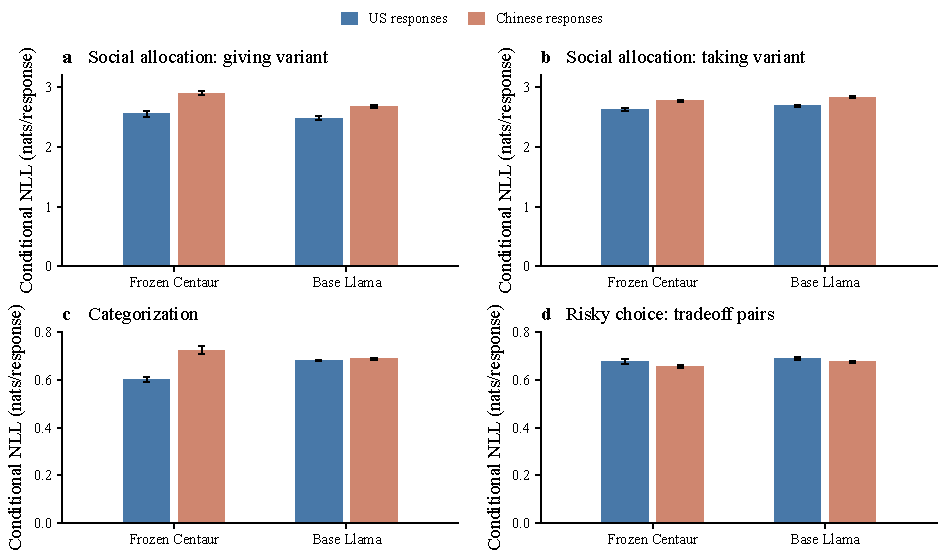
\includegraphics[width=\textwidth]{figures/frozen_sample_fit.pdf}
\caption{Frozen Centaur and Llama prediction error by population (H1); lower is better. Giving uses held-out participants, Taking a separate sample, and the other tasks all retained participants. Allocation bars have 95\% participant-bootstrap intervals; the newer tasks are descriptive. Category choice covers 15 items; lotteries cover four tradeoff pairs. Scores are conditional on valid responses and should be compared within each task.}
\label{fig:frozen}
\end{figure}

\subsection{H2: fine-tuning population changes predictions}
\begin{itemize}
\item Clear prediction shifts on unseen items in all three datasets (Figures~\ref{fig:population} and~\ref{fig:transfer}).
\item After US fine-tuning, the model predicts more category choices. After Chinese fine-tuning, it predicts more 10-point lottery choices, especially on tradeoff items.
\item Within the same task, fine-tuning on the matching population usually predicts its responses better than fine-tuning on the other population. It doesn't always beat frozen Centaur.
\item Size of the differences: China fine-tuning improves Giving log score for held-out Chinese responses by 0.144 nats over US fine-tuning (95\% CI 0.105--0.179). Compared with China fine-tuning, US fine-tuning predicts 26.6 percentage points more category choices and 21.5 points fewer 10-point lottery choices on tradeoff pairs. Participant uncertainty for these last two estimates is still missing.
\end{itemize}




\begin{figure}[H]
\centering
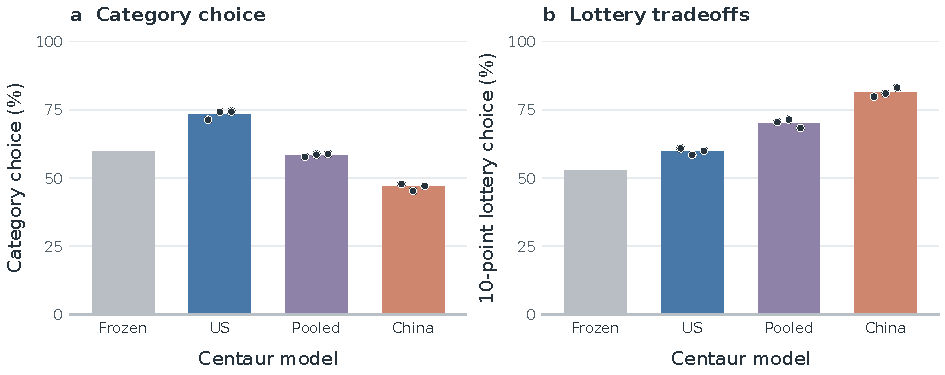
\includegraphics[width=\textwidth]{figures/population_predictions.pdf}
\caption{Fine-tuning population shifts predictions on unseen items (H2). Bars show category-choice probability across 15 items and 10-point choice probability across four lottery tradeoffs. Pooled fine-tuning uses equal numbers of US and Chinese participants. Dots show three seeds; predictions average both answer orders. Lottery fine-tuning includes dominance items as well. These shifts do not measure accuracy.}
\label{fig:population}
\end{figure}

\subsection{H3: shifts carry over to Taking, but don't consistently match human differences}
\begin{itemize}
\item Fine-tuning only on Giving also changes Taking predictions (Figures~\ref{fig:transfer} and~\ref{fig:social}). The differences between fine-tuning populations carry over to this new task.
\item On Taking, the difference between adapters goes in the opposite direction to the human US--China difference when both study waves are combined. The human difference also changes across waves.
\item The US adapter predicts both Taking populations better. Matching the fine-tuning and test populations doesn't consistently help on the new task.
\item Fewer tokens mean less generosity in Giving but more generosity in Taking. The same numerical shift can mean different behavior.
\item \textbf{Figure still missing:} human US--China differences next to the differences between adapters, for all 25 targets. Giving and Taking shown separately, with human data split by wave and held-out participants used for Giving. The model comparison uses the same adapters, fitted across waves. Differences and uncertainty shown on the same response scale. The five groups below are examples.
\end{itemize}


\begin{figure}[H]
\centering
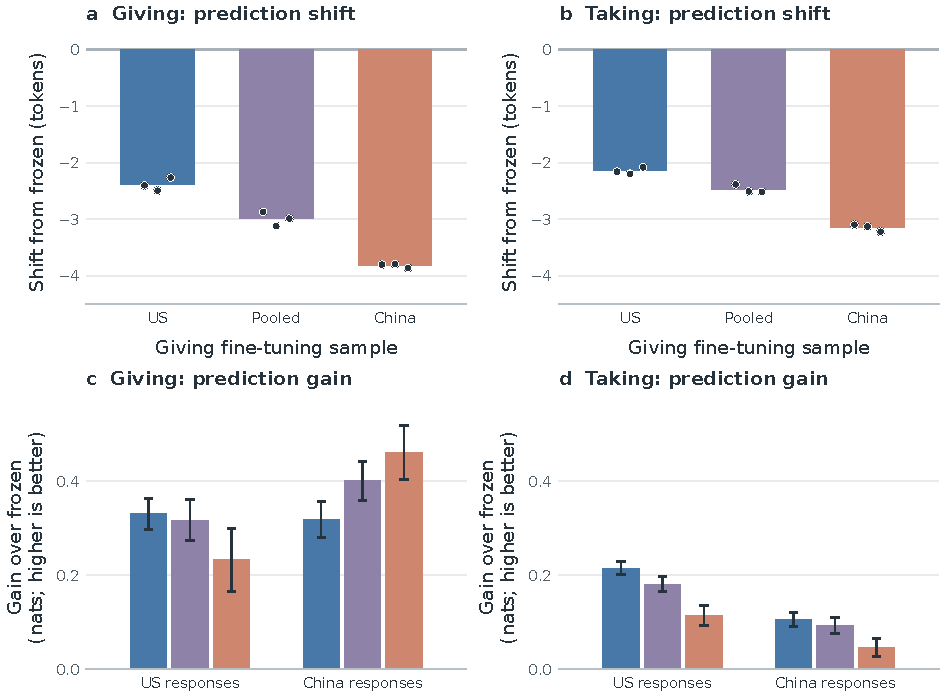
\includegraphics[width=\textwidth]{figures/giving_taking_population_effects.pdf}
\caption{How fine-tuning on Giving changes Giving and Taking (H2--H3). Top: change in expected tokens from frozen Centaur; dots show three seeds. Bottom: prediction gain over frozen Centaur for each population; bars have 95\% paired participant-and-seed bootstrap intervals. All conditions use equal data budgets and held-out targets. Taking is never used for fine-tuning. A negative shift means less giving but also less taking, so its meaning for generosity differs between tasks.}
\label{fig:transfer}
\end{figure}

\begin{figure}[H]
\centering
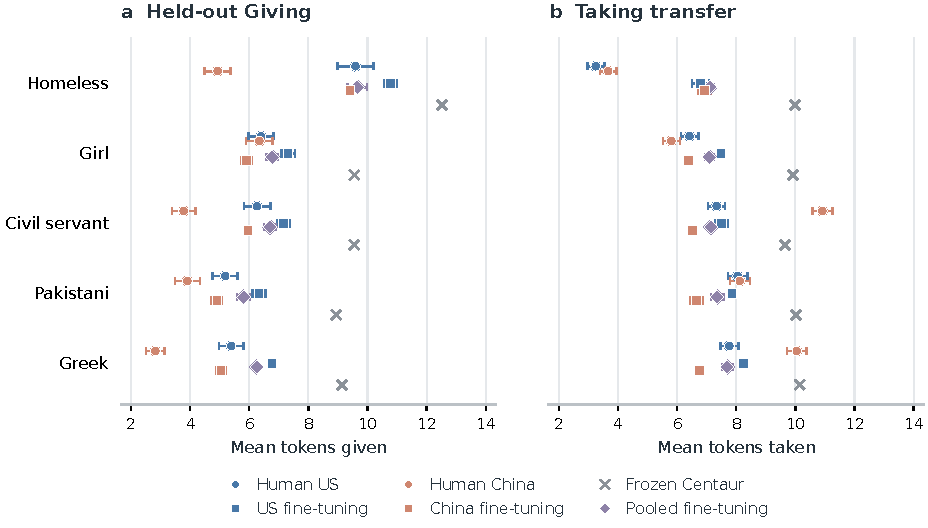
\includegraphics[width=\textwidth]{figures/social_group_predictions.pdf}
\caption{Human responses and model predictions for five illustrative social groups (H2--H3). Both panels use adapters fine-tuned only on Giving, with the plotted target held out. Circles show human means; squares show US and China fine-tuning; diamonds show pooled fine-tuning; crosses show frozen Centaur. Human intervals are 95\% participant-bootstrap intervals; model intervals show one standard deviation across three seeds. The selected groups illustrate the patterns; they are not a test across all targets.}
\label{fig:social}
\end{figure}

\subsection{H4: fine-tuning adds more than a response adjustment in some cases}
\begin{itemize}
\item Categorization: fine-tuning adds little consistent benefit over the simple response adjustment.
\item Taking: fine-tuning usually does better than the adjustment. Lottery tradeoffs: mixed results, depending on who the model was fine-tuned on and who it predicts (Figure~\ref{fig:adjustment}).
\item Answer order has a large effect. Some remaining gains may come from correcting answer preferences. We don't yet know whether they reflect richer learning about behavior.
\end{itemize}

\begin{figure}[H]
\centering
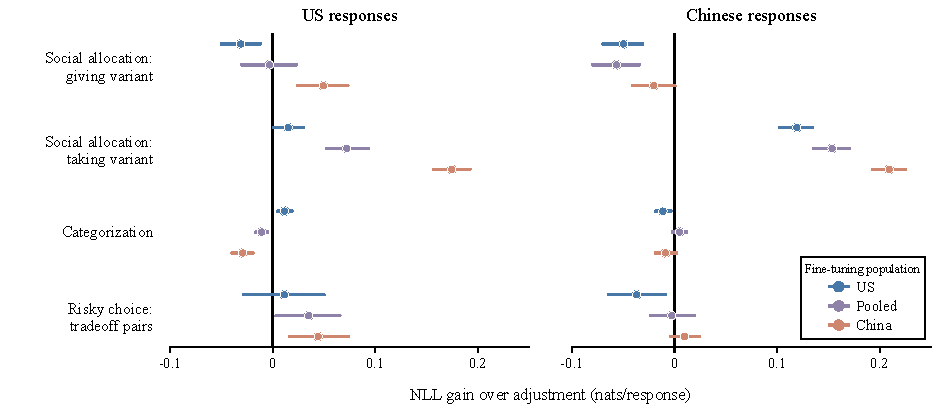
\includegraphics[width=\textwidth]{figures/response_adjustment_comparison.pdf}
\caption{Fine-tuning compared with a response adjustment fitted to the same data (H4). Positive values favor fine-tuning. Both methods use Giving data for the top panels, category choices for the bottom left, and lottery choices for the bottom right. The adjustment changes response preferences shared across items while model weights stay fixed. Error bars show 95\% paired participant-and-seed bootstrap intervals for allocation tasks; dots show three seeds for the newer tasks. Lottery results cover tradeoffs only. Answer-position calibration remains to be checked.}
\label{fig:adjustment}
\end{figure}
